\documentclass[11pt]{article}

\usepackage[paperheight=9in,paperwidth=6in]{geometry}
\pagenumbering{gobble}
\usepackage{fontspec}
\setmainfont{EB Garamond}[UprightFont=EB Garamond Regular,
ItalicFont= EB Garamond Italic,
BoldFont= EB Garamond Bold,
Ligatures=Rare,
StylisticSet=6,
Numbers=Proportional,
Numbers=OldStyle]
%\usepackage{graphicx}
\usepackage[autocompile]{gregoriotex}
\def\GreStar{*}
\def\GreDagger{†}


\begin{document}
%\begin{titlepage}
% \begin{center}
% \fontsize{36}{45}\selectfont{D\textsc{ominica}\\ A\textsc{d} V\textsc{esperas}}
% \end{center}
%\centering
%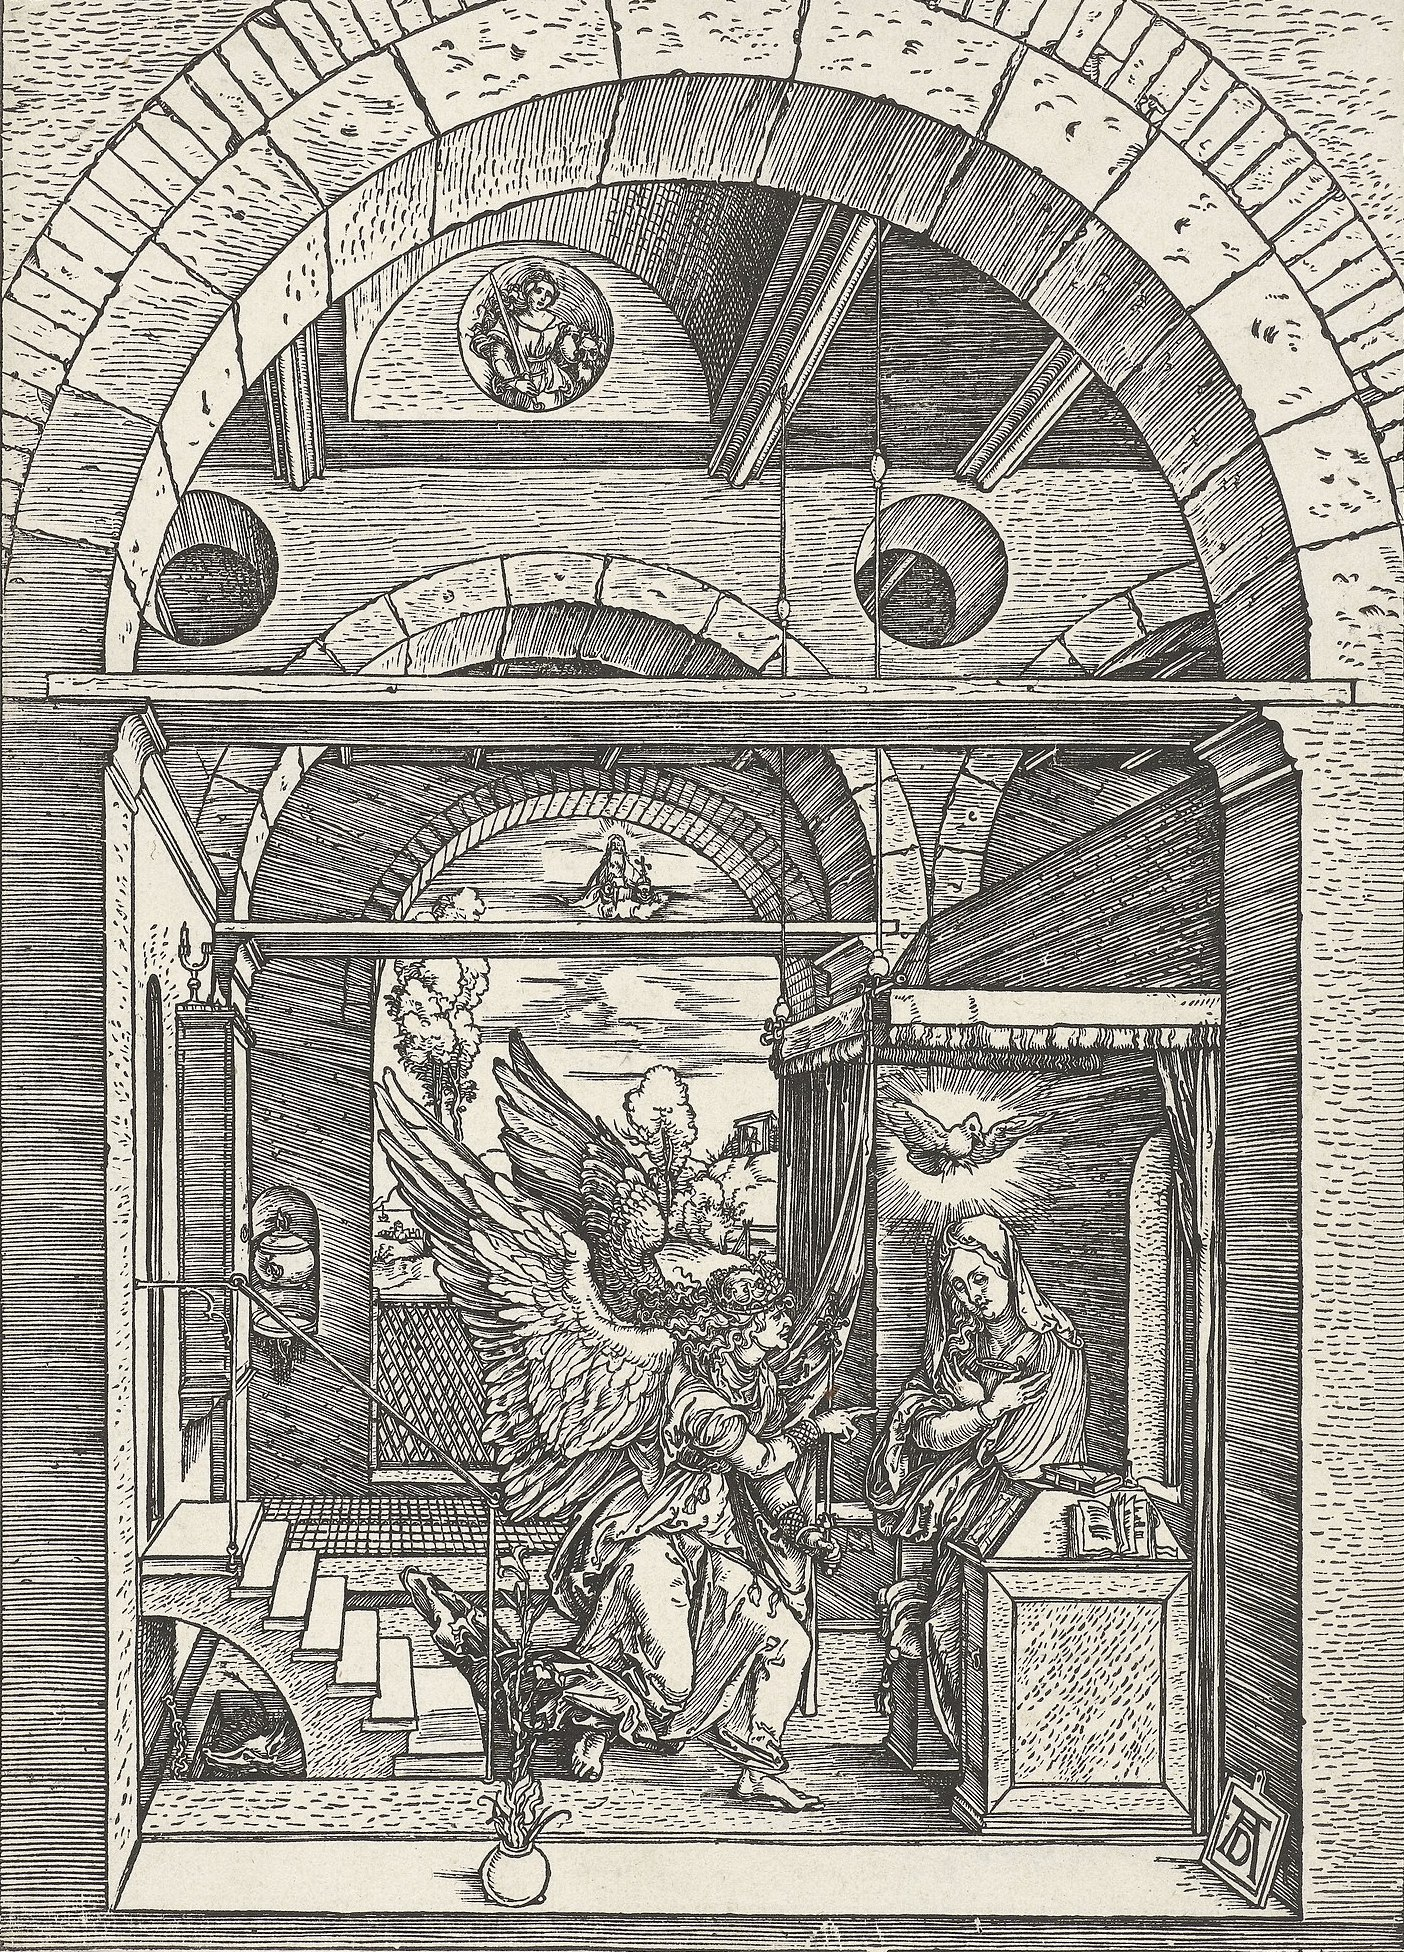
\includegraphics[width=10cm,height=10cm,keepaspectratio]{Annunciatie_Leven_van_Maria_(serietitel),_RP-P-OB-1406}
%\begin{center}
% \fontsize{36}{45}\selectfont{T\textsc{empore} A\textsc{dventus}}
%\end{center}
%\end{titlepage}
%\newpage\null\thispagestyle{empty}\newpage

\begin{center}Sabbato ante Dominicam I Adventus\end{center}

\begin{center}
Ad Vesperas
\end{center}

\textit{Psalmi de Sabbato. Antiphone de Vesperis Dominicae sequentis.}

\begin{center}Capitulum.\end{center}

\begin{flushright}{Rom. 13:11}\end{flushright}
Fratres: Hora est jam nos de somno súrgere: † nunc enim própior est nostra salus, * quam cum credídimus.

℟. Deo grátias.

\vspace{2mm}
\textit{Sic semper respondetur in fine omnium Capitulorum.}
\begin{center}{Hymnus}\end{center}
\greannotation{4.}
\grechangestyle{initial}{\fontsize{32}{32}\selectfont}
\gregorioscore{Creator_alme_siderum.gabc}
\bigskip

\def\GreStar{*}
\gresetinitiallines{0}
\gregorioscore{Versus_in_Adventu}
\noindent \hspace*{-0,2mm} ℟ . \hspace{2mm}Aperiátur \hspace{1.1mm}térra, \hspace{1.9mm}et \hspace{3.9mm}gérminet \hspace{5.5mm}Salvató- \hspace{4mm}rem.

\gresetinitiallines{1}
\greannotation{Ad Magnif.}
\greannotation{Ant. 1. f}
\grechangedim{annotationraise}{0.05 mm}{scalable}
\grechangestyle{initial}{\fontsize{32}{32}\selectfont}
\gregorioscore{Ecce_nomen_Domini}

\vspace{2mm}
\textit{Oratio ut infra ad Vesperas Dominicae.}
\vspace{2mm}

\textit{Suffragium de Omnibus Sanctis non fit per totum Adventum.}

\textit{In Adventum non fit de Festo nisi fuerit Duplex vel Semiduplex. Duplex I classis, si occurat in Dominica I. Adventus, transfertur: si in aliis Dominicis fit de eo cum commemoratione Dominicae. Duplex vero II. classis occurens in Dominica quacumque Adventus transfertur juxta Rubricas.}

\textit{De quocumque alio Duplici vel Semiduplici occurente in Dominica fit tantum commemoratio in utrisque Vesperis. De Simplici fit tantum commmemoratio etiam in Feriis.}

\begin{center}Dominica I Adventus\end{center}

\begin{center}
Ad Vesperas
\end{center}

\textit{Antiphonae propriae ut infra. Psalmi de Dominica. Capitulum et Hymnus ut in I Vesperis.}

\greannotation{1. Ant.}
\greannotation{8. G}
\grechangestyle{initial}{\fontsize{32}{32}\selectfont}
\gregorioscore{In_illa_die}

\greannotation{2. Ant.}
\greannotation{8. G\textsuperscript{*}}
\grechangestyle{initial}{\fontsize{31}{31}\selectfont}
\gregorioscore{Jucundare}

\greannotation{3. Ant.}
\greannotation{5. a}
\grechangestyle{initial}{\fontsize{32}{32}\selectfont}
\gregorioscore{Ecce_dominus_veniet}

\greannotation{4. Ant.}
\greannotation{7. c}
\grechangestyle{initial}{\fontsize{32}{32}\selectfont}
\gregorioscore{Omnes_sitientes}

\greannotation{5. Ant.}
\greannotation{4. A\textsuperscript{*}}
\grechangedim{annotationraise}{0.03 mm}{scalable}
\grechangestyle{initial}{\fontsize{32}{32}\selectfont}
\gregorioscore{Ecce_veniet_propheta}

\greannotation{Ad Magnif.}
\greannotation{Ant. 8. G}
\grechangedim{annotationraise}{0.03 mm}{scalable}
\grechangestyle{initial}{\fontsize{32}{32}\selectfont}
\gregorioscore{Ne_timeas_maria_Alleluia}


\begin{center}Oratio\end{center}

Orémus.\\
Excita, quǽsumus, Dómine, poténtiam tuam, et veni: † ut ab imminéntibus peccatórum nostrórum perículis, te mereámur protegénte éripi, * te liberánte salvári. Qui vivis et regnas cum Deo Patre, in unitáte Spíritus Sancti, Deus,* per ómnia sǽcula sæculórum.

℟. Amen.

\vspace{2mm}
\textit{Hymnus} et ℣. \textit{et hujus Dominicae dicuntur in aliis Dominicis et in Feriis Adventus.}
\bigskip
\enddocument